\documentclass[a4paper, 11pt]{article}
\usepackage[francais]{babel}
\usepackage[margin=3cm]{geometry}
\usepackage[utf8]{inputenc} 
\usepackage{amsmath}
\usepackage{amssymb}
\usepackage{graphicx}

\title{Calcul de valeurs d'arguments. Cahier des Charges}
\author{Edouard Delasalles, Thomas Gerald, Alexis Martin}



\begin{document}
\maketitle
\section*{Introduction}
L'objectif du projet est de créer un logiciel extensible et modulable d'aide à l'analyse de graphes d'arguments. Le logiciel devra supporter différent types de graphes, avec différent paramètres sur les arcs(attaque et soutient) et les nœuds (valeurs, tags, etc...), et proposer plusieurs algorithmes.

\section{Représentation des données}
Le graphe sera capable de supporter plusieurs types de paramètres sur ses arcs et sur ses nœuds, pouvant servir ou non à l'exécution des algorithmes. Il sera possible de créer, sauvegarder, lire un graphe. Pouvoir importer des graphes depuis la plate-forme web debategraph serait aussi un plus. \\

\section{Fonctionnalités}
Les algorithmes implémentés dans l'outil serviront à extraire des informations sur les graphes d'arguments passés en entrés. Ces informations, les arguments les plus controversés ou les plus soutenus par exemple, pourront servir à l'analyse du graphe par l'utilisateur. Le logiciel donnera aussi des outils à l'utilisateur qui lui permettront de comparer les différents algorithmes afin de pouvoir choisir lequel répond le plus à ses besoins. \\

Le logiciel sera doté de 5 algorithmes de résolution :
\begin{itemize}
\item[•]Catégoriser
\item[•]Social Abstract Argumentation Framework (paramétré par un $\epsilon$)
\item[•]Discussion-based semantics
\item[•]Burden-based semantics (paramétré par un $\epsilon$)
\item[•]Propagation\\
\end{itemize}

Dans une version avancé, l'outil sera aussi capable de proposer l'ajout d’algorithmes par l'utilisateur de manière simplifiée, via une interface graphique ou une API par exemple.\\

\section{Visualisation}
Le logiciel sera aussi doté d'un système de visualisation interactif des graphes d’arguments. L'utilisateur pourra ainsi visualiser un graphe doté de différents paramètres, ré-arranger la topographie des nœuds et des arcs. De plus, les résultats des algorithmes pourront également être affichés, via un code couleur par exemple (Nous projetons d'utiliser la bibliothèque graphstream). 

Une première visualisation du rendu final est présentée dans la figure \ref{image}. \\

Une documentation sur l'utilisation du logiciel sera fourni afin d'orienter l'utilisateur dans l'utilisation de ce dernier.\\

\begin{figure}[h]
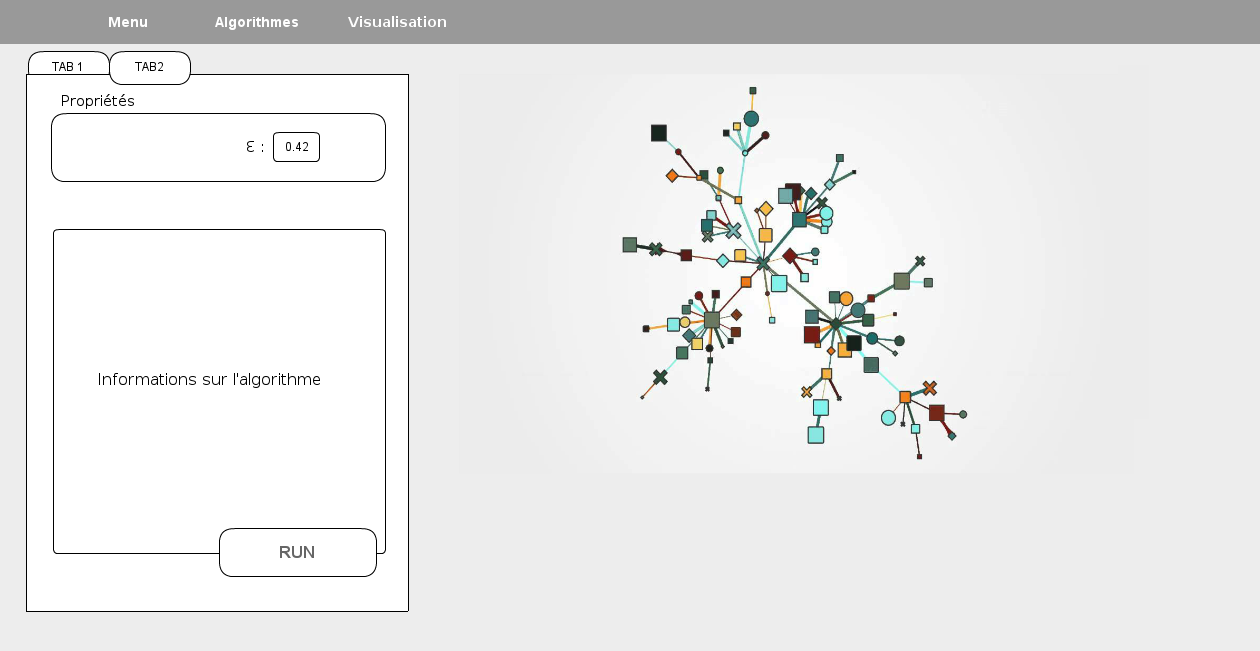
\includegraphics[width=13cm]{Wireframe.png}
\caption{Ébauche d'interface pouvant être créée.}
\label{image}
\end{figure}

\section{Calendrier prévisionnel}

\begin{description}
\item[Structure et implémentation des graphes: ] deadline le 15 mars.
\item[Structure et implémentation des algorithmes: ] deadline le 29 mars.
\item[Interface: ] deadline le 12 avril.
\item[Tests et analyses: ] deadline le 26 avril.
\item[Rendu du projet et de la synthèse: ] deadline le 8 mai.


\end{description}

\end{document}